% Editable reconstruction; interpretation recorded in root.json.
% Shared standalone design for the editable figure reconstructions.
\documentclass[tikz,border=5pt,10pt]{standalone}
\usepackage[T1]{fontenc}
\usepackage[utf8]{inputenc}
\usepackage{newpxtext,newpxmath}
\usepackage[scaled=.94]{sourcesanspro}
\usepackage{pgfplots}
\pgfplotsset{compat=1.18}
\usetikzlibrary{arrows.meta,calc,positioning,decorations.pathreplacing,
  decorations.markings,patterns,matrix,shapes.geometric,fit,backgrounds,
  intersections,angles,quotes}
\definecolor{ink}{HTML}{203746}
\definecolor{accent}{HTML}{146C78}
\definecolor{muted}{HTML}{667780}
\definecolor{signalred}{HTML}{B94B44}
\color{ink}
\tikzset{>=Latex,line width=.8pt,
  every node/.style={font=\small},
  axis/.style={->,draw=muted,line width=.5pt},
  guide/.style={draw=muted,dashed,line width=.45pt},
  curve/.style={draw=accent,line width=1pt},
  marker/.style={circle,fill=accent,inner sep=1.5pt},
  labelbox/.style={fill=white,inner sep=2pt}}

\begin{document}

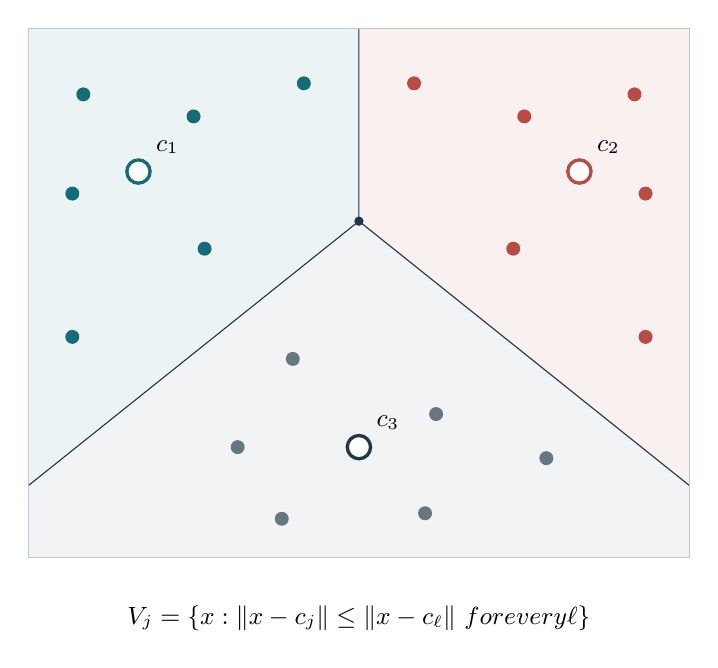
\begin{tikzpicture}[scale=1.4]
\fill[accent!8] (-3,-1.85)--(0,.55)--(0,2.3)--(-3,2.3)--cycle;
\fill[signalred!8] (0,.55)--(3,-1.85)--(3,2.3)--(0,2.3)--cycle;
\fill[muted!9] (-3,-2.5)--(3,-2.5)--(3,-1.85)--(0,.55)--(-3,-1.85)--cycle;
\draw[ink] (-3,-1.85)--(0,.55)--(3,-1.85) (0,.55)--(0,2.3);
\draw[muted!40] (-3,-2.5) rectangle (3,2.3);
\foreach \p in {(-2.6,.8),(-2.5,1.7),(-1.5,1.5),(-1.4,.3),(-2.6,-.5),(-.5,1.8)}{\fill[accent] \p circle(1.8pt);}
\foreach \p in {(2.6,.8),(2.5,1.7),(1.5,1.5),(1.4,.3),(2.6,-.5),(.5,1.8)}{\fill[signalred] \p circle(1.8pt);}
\foreach \p in {(-1.1,-1.5),(-.6,-.7),(.7,-1.2),(.6,-2.1),(-.7,-2.15),(1.7,-1.6)}{\fill[muted] \p circle(1.8pt);}
\foreach \p/\lab/\col in {(-2,1)/c_1/accent,(2,1)/c_2/signalred,(0,-1.5)/c_3/ink}{\draw[\col,line width=1.2pt,fill=white] \p circle(3pt);\node[above right=4pt] at \p {$\lab$};}
\fill[ink] (0,.55) circle(1.2pt);
\node at (0,-3.05) {$\displaystyle V_j=\{x:\|x-c_j\|\leq\|x-c_\ell\|\ \text{for every }\ell\}$};
\end{tikzpicture}
\end{document}
